\documentclass{article}

%%%%%%%%%%%%%%%%%%%%%%%%%%%%%%%%%%%%%%%%%
% Lachaise Assignment
% Structure Specification File
% Version 1.0 (26/6/2018)
%
% This template originates from:
% http://www.LaTeXTemplates.com
%
% Authors:
% Marion Lachaise & François Févotte
% Vel (vel@LaTeXTemplates.com)
%
% License:
% CC BY-NC-SA 3.0 (http://creativecommons.org/licenses/by-nc-sa/3.0/)
% 
%%%%%%%%%%%%%%%%%%%%%%%%%%%%%%%%%%%%%%%%%

%----------------------------------------------------------------------------------------
%	PACKAGES AND OTHER DOCUMENT CONFIGURATIONS
%----------------------------------------------------------------------------------------

\usepackage{amsmath,amsfonts,stmaryrd,amssymb} % Math packages

\usepackage{enumerate} % Custom item numbers for enumerations

\usepackage[ruled]{algorithm2e} % Algorithms

\usepackage[framemethod=tikz]{mdframed} % Allows defining custom boxed/framed environments

\usepackage{listings} % File listings, with syntax highlighting
\lstset{
	basicstyle=\ttfamily, % Typeset listings in monospace font
}

%----------------------------------------------------------------------------------------
%	DOCUMENT MARGINS
%----------------------------------------------------------------------------------------

\usepackage{geometry} % Required for adjusting page dimensions and margins

\geometry{
	paper=a4paper, % Paper size, change to letterpaper for US letter size
	top=2.5cm, % Top margin
	bottom=3cm, % Bottom margin
	left=2.5cm, % Left margin
	right=2.5cm, % Right margin
	headheight=14pt, % Header height
	footskip=1.5cm, % Space from the bottom margin to the baseline of the footer
	headsep=1.2cm, % Space from the top margin to the baseline of the header
	%showframe, % Uncomment to show how the type block is set on the page
}

%----------------------------------------------------------------------------------------
%	FONTS
%----------------------------------------------------------------------------------------

\usepackage[utf8]{inputenc} % Required for inputting international characters
\usepackage[T1]{fontenc} % Output font encoding for international characters
\usepackage{listings}
\usepackage{color}
\usepackage{float}


\definecolor{mygreen}{rgb}{0,0.6,0}
\definecolor{mygray}{rgb}{0.5,0.5,0.5}
\definecolor{mymauve}{rgb}{0.58,0,0.82}

\lstset{ 
  backgroundcolor=\color{white},   % choose the background color; you must add \usepackage{color} or \usepackage{xcolor}; should come as last argument
  basicstyle=\footnotesize,        % the size of the fonts that are used for the code
  breakatwhitespace=false,         % sets if automatic breaks should only happen at whitespace
  breaklines=true,                 % sets automatic line breaking
  captionpos=b,                    % sets the caption-position to bottom
  commentstyle=\color{mygreen},    % comment style
  deletekeywords={...},            % if you want to delete keywords from the given language
  escapeinside={\%*}{*)},          % if you want to add LaTeX within your code
  extendedchars=true,              % lets you use non-ASCII characters; for 8-bits encodings only, does not work with UTF-8
  firstnumber=1000,                % start line enumeration with line 1000
  frame=single,	                   % adds a frame around the code
  keepspaces=true,                 % keeps spaces in text, useful for keeping indentation of code (possibly needs columns=flexible)
  keywordstyle=\color{blue},       % keyword style
  language=C,                 % the language of the code
  morekeywords={*,...},            % if you want to add more keywords to the set
  rulecolor=\color{black},         % if not set, the frame-color may be changed on line-breaks within not-black text (e.g. comments (green here))
  showspaces=false,                % show spaces everywhere adding particular underscores; it overrides 'showstringspaces'
  showstringspaces=false,          % underline spaces within strings only
  showtabs=false,                  % show tabs within strings adding particular underscores
  stepnumber=2,                    % the step between two line-numbers. If it's 1, each line will be numbered
  stringstyle=\color{mymauve},     % string literal style
  tabsize=4,	                   % sets default tabsize to 2 spaces
  title=\lstname                   % show the filename of files included with \lstinputlisting; also try caption instead of title
}


%
%----------------------------------------------------------------------------------------
%	COMMAND LINE ENVIRONMENT
%----------------------------------------------------------------------------------------

% Usage:
% \begin{commandline}
%	\begin{verbatim}
%		$ ls
%		
%		Applications	Desktop	...
%	\end{verbatim}
% \end{commandline}

\mdfdefinestyle{commandline}{
	leftmargin=10pt,
	rightmargin=10pt,
	innerleftmargin=15pt,
	middlelinecolor=black!50!white,
	middlelinewidth=2pt,
	frametitlerule=false,
	backgroundcolor=black!5!white,
	frametitle={Command Line},
	frametitlefont={\normalfont\sffamily\color{white}\hspace{-1em}},
	frametitlebackgroundcolor=black!50!white,
	nobreak,
}

% Define a custom environment for command-line snapshots
\newenvironment{commandline}{
	\medskip
	\begin{mdframed}[style=commandline]
}{
	\end{mdframed}
	\medskip
}

%----------------------------------------------------------------------------------------
%	FILE CONTENTS ENVIRONMENT
%----------------------------------------------------------------------------------------

% Usage:
% \begin{file}[optional filename, defaults to "File"]
%	File contents, for example, with a listings environment
% \end{file}

\mdfdefinestyle{file}{
	innertopmargin=1.6\baselineskip,
	innerbottommargin=0.8\baselineskip,
	topline=false, bottomline=false,
	leftline=false, rightline=false,
	leftmargin=2cm,
	rightmargin=2cm,
	singleextra={%
		\draw[fill=black!10!white](P)++(0,-1.2em)rectangle(P-|O);
		\node[anchor=north west]
		at(P-|O){\ttfamily\mdfilename};
		%
		\def\l{3em}
		\draw(O-|P)++(-\l,0)--++(\l,\l)--(P)--(P-|O)--(O)--cycle;
		\draw(O-|P)++(-\l,0)--++(0,\l)--++(\l,0);
	},
	nobreak,
}

% Define a custom environment for file contents
\newenvironment{file}[1][File]{ % Set the default filename to "File"
	\medskip
	\newcommand{\mdfilename}{#1}
	\begin{mdframed}[style=file]
}{
	\end{mdframed}
	\medskip
}

%----------------------------------------------------------------------------------------
%	NUMBERED QUESTIONS ENVIRONMENT
%----------------------------------------------------------------------------------------

% Usage:
% \begin{question}[optional title]
%	Question contents
% \end{question}

\mdfdefinestyle{question}{
	innertopmargin=1.2\baselineskip,
	innerbottommargin=0.8\baselineskip,
	roundcorner=5pt,
	nobreak,
	singleextra={%
		\draw(P-|O)node[xshift=1em,anchor=west,fill=white,draw,rounded corners=5pt]{%
		Question \theQuestion\questionTitle};
	},
}

\newcounter{Question} % Stores the current question number that gets iterated with each new question

% Define a custom environment for numbered questions
\newenvironment{question}[1][\unskip]{
	\bigskip
	\stepcounter{Question}
	\newcommand{\questionTitle}{~#1}
	\begin{mdframed}[style=question]
}{
	\end{mdframed}
	\medskip
}

%----------------------------------------------------------------------------------------
%	WARNING TEXT ENVIRONMENT
%----------------------------------------------------------------------------------------

% Usage:
% \begin{warn}[optional title, defaults to "Warning:"]
%	Contents
% \end{warn}

\mdfdefinestyle{warning}{
	topline=false, bottomline=false,
	leftline=false, rightline=false,
	nobreak,
	singleextra={%
		\draw(P-|O)++(-0.5em,0)node(tmp1){};
		\draw(P-|O)++(0.5em,0)node(tmp2){};
		\fill[black,rotate around={45:(P-|O)}](tmp1)rectangle(tmp2);
		\node at(P-|O){\color{white}\scriptsize\bf !};
		\draw[very thick](P-|O)++(0,-1em)--(O);%--(O-|P);
	}
}

% Define a custom environment for warning text
\newenvironment{warn}[1][Warning:]{ % Set the default warning to "Warning:"
	\medskip
	\begin{mdframed}[style=warning]
		\noindent{\textbf{#1}}
}{
	\end{mdframed}
}

%----------------------------------------------------------------------------------------
%	INFORMATION ENVIRONMENT
%----------------------------------------------------------------------------------------

% Usage:
% \begin{info}[optional title, defaults to "Info:"]
% 	contents
% 	\end{info}

\mdfdefinestyle{info}{%
	topline=false, bottomline=false,
	leftline=false, rightline=false,
	nobreak,
	singleextra={%
		\fill[black](P-|O)circle[radius=0.4em];
		\node at(P-|O){\color{white}\scriptsize\bf i};
		\draw[very thick](P-|O)++(0,-0.8em)--(O);%--(O-|P);
	}
}

% Define a custom environment for information
\newenvironment{info}[1][Info:]{ % Set the default title to "Info:"
	\medskip
	\begin{mdframed}[style=info]
		\noindent{\textbf{#1}}
}{
	\end{mdframed}
}
 % Include the file specifying the document structure and custom commands

%----------------------------------------------------------------------------------------
%	ASSIGNMENT INFORMATION
%----------------------------------------------------------------------------------------

\title{Parallel computing, Programming assignment} % Title of the assignment
\author{Angelos Anagnostopoulos\\ \texttt{up1066593@upnet.gr}} % Author name and email address
\date{University of Patras --- \today} % University, school and/or department name(s) and a date

%----------------------------------------------------------------------------------------

\begin{document}

\maketitle % Print the title

%----------------------------------------------------------------------------------------
%	INTRODUCTION
%----------------------------------------------------------------------------------------

\section*{Introduction} % Unnumbered section

The point of this excercise was to use parallelization libraries in the C programming language in order to calculate various numbers with use of different algorithms and mathematical formulae. 
Code was written in both OpenMP and the MPI libraries, both wrappers that deal with threads and inter-process messages. 
They are very easy to use and replace the mind-bending complexity of Posix threads, and thus were embraced by the C community. 

For this assignment, we have to calculate the constants e and $ \pi $, as well as the natural logarithm $ \ln $(x) of a small number x between 0 and 2.

%----------------------------------------------------------------------------------------
%	PROBLEM 1: Approximating pi
%----------------------------------------------------------------------------------------

\section{Approximating pi} % Numbered section

Throughout the years, multiple methods of approximating $ \pi $ have been proposed, each with its own pros and cons.
For this assignment we were left free to choose the implementation details by ourselves,
which gives us room to navigate into different mathematical formulae and write some interesting code.

\subsection{OpenMP implementation}

By integrating $ \sqrt{1-x^2}	$ from -1 to 1 we can calculate the value of pi wiht great accuracy.
This stems from the fact that the integral converges to $ \frac{\pi}{2} $. We therefore need to arithmetically calculate the integral:
\begin{equation}
	I = \int_{-1}^{1} \sqrt{1-x^2} \; \text{d}x = \frac{\pi}{2}.
\end{equation}

Arithmetic integration is done by using a tiny step dx in order to divide the integral up into very small areas that can be calculated and summed up. We divide our function f(x) into multiple dx segments and multiply the function value with our current dx segment, adding the result to a "master" sum.
This is essentialy the definition of a definite integral. The smaller we make dx, the better the accuracy of the method. As it turns out, even relatively small values of 10.000, are effective in calculating multiple decimal points. As we will see later on, this is not the case with our other method of choice. The complete source code can be seen on the next page.

In each itteration of the program, for each small dx we add a partial area value to the result. At the end we display the final result to the console. With a standard integer we can reach about 2 million itterations, which is more than enough to calculate $ \pi $ with great accuracy.

\newpage
\lstinputlisting[language=C]{"/home/angelos/Desktop/parallel_projects/pi_aprox/pi_integral_openmp.c"}

%------------------------------------------------

\subsection{MPI implementation}

The MPI library is a bit more complicated syntactically, but ultimatelly achieves the same results by allowing different threads and processes to communicate with each other and automatically dividing the workload to them.
For this method, we chose to implement a Monte Carlo method. By using randomness over many itterations, we can reach an estimation about the value of $ \pi $ which is close to the real thing!

This of course requires creation of a random number in each itteration and is very time consuming but yeilds promising results for large numbers of itterations.
For our needs, we went with 10.000.000. Unfortunately this number does not give us accurate results, so a workaround has been implemented.
By storing calculated values in a file and taking their median, we can come a lot closer to the true value of $ \pi $ than with a single use of the method.

Our method is based on the unit circle, and the fact that the area under one quarter of the unit circle is equal to $ \frac{\pi}{4} $. By taking a lot of random points and seeing if they belong inside the unit circle or not, we can come up with a clever trick to calculate an approximation of pi as the number of "hits" divided by the total number of points.
Let the total number of points be N and the points inside the unit circle M. Then:
\begin{align}
	\frac{M}{N} = \frac{\pi}{4},\\
	\pi = \frac{4 * M}{N}
\end{align}
After writting the results to the file, a small python script is called to calculate the median and print the output to the screen. Below is the source code for the MPI implementation as well as the python script:
\newpage
\begin{center}
	Approximating $ \pi $ with MPI source code
\end{center}
\lstinputlisting[language=C]{"/home/angelos/Desktop/parallel_projects/pi_aprox/pi_montecarlo_MPI.c"}
\newpage
\begin{center}
	Python script to find median of multiple approximations
\end{center}
\lstinputlisting[language=Python]{"/home/angelos/Desktop/parallel_projects/pi_aprox/sumfile.py"}

In order to automate the whole process, a shell script was created. To run it, simply execute:
\begin{lstlisting}[language=bash]
	$ ./pi_aprox/run.sh
\end{lstlisting}


%----------------------------------------------------------------------------------------
%	PROBLEM 2: Approximating ln(x)
%----------------------------------------------------------------------------------------

\section{Approximating ln(x)}

In order to approximate the value of ln(x), we can use a mathematical formula derived by the Taylor series.
That will give us a sum that we shall divide upon our threads to calculate partially, and then add their results to a master-sum.
The formula in question is:
\begin{equation}
	ln(x) = \sum_{i=1}^{n}(-1)^{i+1}[\frac{(x-1)^i}{i}]
\end{equation}
\newline
\begin{center}
	Natural logarithm ln(x) approximation source code:
\end{center}

\lstinputlisting[language=C]{"/home/angelos/Desktop/parallel_projects/ln_aprox/ln_openmp.c"}

%----------------------------------------------------------------------------------------
%	PROBLEM 3: Approximating e
%----------------------------------------------------------------------------------------

\section{Approximating e}

Euler's constant can be calculated from the McLauren series:
\begin{equation}
	e = \sum_{n=0}^{\infty}\frac{1}{n!}
\end{equation}
We shall create an algorithm that parallelizes this, exactly as we did with ln(x) in the above section.
This algorithm will need to calculate the factorial of each itteration and add the partial sum to our approximation of e.
\begin{center}
	Euler's constant (e) approximation source code:
\end{center}
\lstinputlisting[language=C]{"/home/angelos/Desktop/parallel_projects/euler_aprox/euler_openmp.c"}


%----------------------------------------------------------------------------------------
\newpage
\section*{Running the code} % Unnumbered section

Shell scripts were created in order to automate file compilation and execution. In order to compile our .c files,simply run:
\begin{lstlisting}[language=bash]
	$ ./compile
\end{lstlisting}

The binary files created, are placed in a new directory called /bin and can be executed with the appropriate command. 
No code has been written to handle wrong/corrupted data, so please input the required parameters properly.
Please note that all code is written with argv in mind for the required steps and the threads to be used. Steps are multiplied by 10.000 for user ease, therefore execute the output with:
\begin{lstlisting}[language=bash]
	./bin/<binary> <steps> <threads_number>
\end{lstlisting}
Only exception is the binary of the natural logarithm approximation,
in which we need to specify a value for x between [0,2]
\begin{lstlisting}[language=bash]
	./bin/ln_openmp <x> <steps> <threads_number>
\end{lstlisting}
\newpage

\section*{Results}

As expected, with more threads comes a major speedup of our calculations, approximately dividing the sequential solution's time by the number of utilised threads.
This division is of course not exact, since spinning up each thread and communicating between them takes some time on its own. Alas, the speedup is quite significant with small numbers of threads.
Were we to go up to batches of 256 or 512 we might see our performance be negatively impacted by further increase in threads number.
Unfortunately, i can only go up to 4 threads so all tests and comparisons were done using 1,2 and 4 of those threads respectively.

Timing code is included in the source code instead of being used with a unix command, so that users can run their own tests and draw their own conclusions on the matter.
The testing machine used is a 4-core intel core-i7 laptop with base frequency of 2.2GHz, and 4KB cache per core. 
A sceencap of timings with different threads/steps combinations is shown bellow:

\begin{center}
	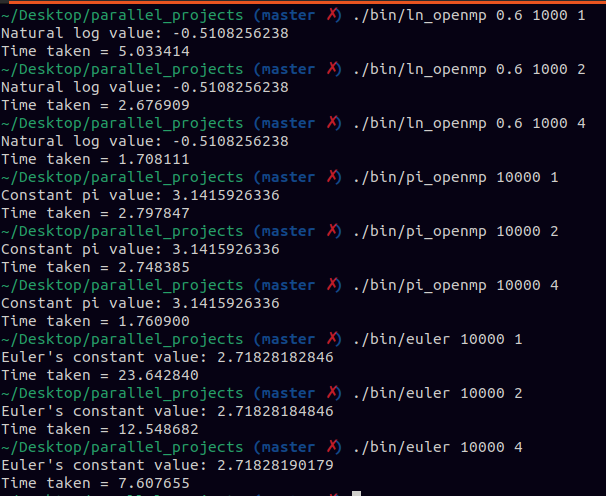
\includegraphics[width=\linewidth]{./benchmarks.png}
	\centering Benchmarks for 1 and 10 million itterations with different numbers of threads.
	
\end{center}

\end{document}
